\lstset{language=awk}

Sérhverju línulegu bestunarverkefni má breyta í svokallað \ath{nykur} (e. dual) verkefni, sem er þá einnig línulegt bestunarverkefni. Einnig kalla \ath{gagnvirkt} verkefni. 

Verkefnin tengjast á þann hátt að lausn á einu verkefni gefur okkur lausnina á hinu. Skuggaverð í frumverkefninu eru ákvörðunarbreytur nykurverkefnisins og öfugt. Stundum er þægi\-legra og hagkvæmara að leysa tilsvarandi nykurverkefni heldur en upphaflega verkefnið.

Gjaldgeng lausn á öðru verkefninu gefur efri (neðri) mörk á bestu lausn hins verkefnisins. 

\begin{daemi}[Efri og neðri mörk]\label{daemi:efrinedrimork}
$$\max_{\vec{x}} z=4x_1+x_2+3x_3 $$
\begin{eqnarray}
x_1+4x_2&\leq&1\\ \label{sk:11}
3x_1-x_2+x_3&\leq&3\\ \label{sk:12}
x_1,x_2,x_3&\geq&0 \nonumber
\end{eqnarray}
\end{daemi}
\begin{lausn}
Ljóst er að sérhver gjaldgeng lausn gefur okkur \emph{neðri mörk} á bestu lausn, t.d. $\vec{x}=(1,0,0)$ gefur $z=4$. Með $\vec{x}=(0,0,3)$ fæst $z=9$. Er þetta seinna gildi nálægt því besta? Til þess að svara því reynum við að finna efri mörk á markfallið.

Margföldum \eqref{sk:11} með 2 og \eqref{sk:12} með 3 og leggjum þær saman (fastar fundnir með ``störun'')
\[\begin{array}{rrrrrrl}
  2(&x_1& +4x_2&& \leq & 1)\\
+ 3(&3x_1&-x_2&+x_3&\leq & 3)\\ \hline
 &  11x_1&+2x_2&+3x_3 &\leq &11
\end{array}\]
Þar sem allar breytur eru $\geq0$ gildir að
$$ \underbrace{4x_1+x_2+3x_3}_{\textrm{markfallið}} \quad \leq \quad \underbrace{11x_1+2x_2+3x_3 \leq 11}_{2\eqref{sk:11}+3\eqref{sk:12}}
$$
þ.e. besta lausn liggur á bilinu $9\leq z^*\leq 11$.

Hægt er að gera enn betur en þetta. Notum breyturnar $y_1$ og $y_2$ í stað fastanna 2 og 3 og finnum þau gildi sem gefa bestu efri mörk. 
\[\begin{array}{rrrrrrl}
  y_1(&x_1& +4x_2&& \leq & 1)\\
+ y_2(&3x_1&-x_2&+x_3&\leq & 3)\\ \hline
 &  (y_1+3y_2)x_1&+(4y_1-y_2)x_2&+(y_2)x_3 &\leq &1(y_1)+3(y_2)
\end{array}\]
Gerum kröfu  um að stuðlar við $x$-in séu a.m.k. jafnstórir og stuðlar markfallsins (svo mörkin haldi), 
\begin{eqnarray*}
 y_1+3y_2 &\geq& 4\\
 4y_1-y_2&\geq&1\\
y_2&\geq&3\\
y_1,y_2&\geq&0
\end{eqnarray*}
Berum nú markfallið saman við þessa summu (og efri mörk hennar)
\begin{eqnarray*}
 z&=&4x_1+x_2+3x_3\\&=&(y_1+3y_2)x_1+(4y_1-y_2)x_2+(y_2)x_3 \\ &\leq &\underbrace{y_1+3y_2}_{\textrm{efri mörk}}
\end{eqnarray*}
Lágmörkum efri mörkin $y_1+3y_2$ með því að leysa
$$ \min_{\vec{y}} w =y_1+3y_2 $$
m.t.t. sk. 
\begin{eqnarray*}
 y_1+3y_2 &\geq& 4\\
 4y_1-y_2&\geq&1\\
y_2&\geq&3\\
y_1,y_2&\geq&0
\end{eqnarray*}
Þetta verkefni kallast \ath{nykur} frumverkefnisins (e. primal). Besta lausn er hægt að leysa myndrænt\footnote{Ef einungis tvær ákvarðanabreytur er um að ræða, þá er einfalt að leysa verkefnið myndrænt.} eða með \textsc{glpk}, 
$$ \vec{y}^*=(y_1^*,y_2^*)=(1,3)\quad\textrm{með}\quad w^*=10.$$
\end{lausn}

\section{Samband frum- og nykurverkefna}
Svarandi til sérhvers línulegs bestunarverkefnis (á stöðluðu formi) 
\[\begin{array}{lcccc}
 \max_{\vec{x}} &z& =& \vec{c}^T\vec{x}\\
 \mbox{sk.}& \vec{A}\vec{x}&\leq&\vec{b}\\
 &\vec{x}&\geq&\vec{0}
\end{array}\quad\Bigg\}\quad\textrm{frum}\]
er nykurverkefnið
\[\begin{array}{lcccc}
 \min_{\vec{y}} &w& =& \vec{b}^T\vec{y}\\
 \mbox{sk.}& \vec{y}^T\vec{A}&\geq&\vec{c}\\
 &\vec{y}&\geq&\vec{0}
\end{array}\quad\Bigg\}\quad\textrm{nykur}\]
Samband frum- og nykurverkefna:

\begin{center}
\begin{tabular}{|ccc|}\hline 
Annað verkefnið && Hitt verkefnið \\ \hline
Skorða $i$ & $\leftrightarrow$ & Breyta $i$ \\
Markfall & $\leftrightarrow$ & Hægri hlið \\
Hámörkun & $\leftrightarrow$ & Lágmörkun  \\ \hline
\end{tabular}
\end{center}

Í dæmi \ref{daemi:efrinedrimork} gaf nykurverkefnið efri mörk á markfalli frumverkefnisins. Almennt gildir:

\begin{setn}[\ath{Veika nykursetningin}\label{setn:veiknykur} (e. weak duality thm.)] Ef $(x_1,...,x_n)$ er leyfileg lausn á frumverkefninu og $(y_1,...,y_m)$ er leyfileg lausn á nykur\-verkefninu, þá er 
$$ \sum_{j=1}^n c_jx_j \leq \sum_{i=1}^m y_ib_i $$ 
\end{setn}
\begin{proof}
\begin{eqnarray*}
 \sum_{j=1}^n c_jx_j &\leq& \sum_{j=1}^n \left(\sum_{i=1}^m y_ia_{ij}\right)x_j \quad\quad\quad(\textrm{því } \vec{y}^T\vec{A}\geq\vec{c})\\
 &=& \sum_{i=1}^m y_i\left(\sum_{j=1}^n a_{ij}x_j\right) \leq \sum_{i=1}^m y_ib_i \quad\quad\quad(\textrm{því } \vec{A}\vec{x}\leq\vec{b})
\end{eqnarray*}
 
\end{proof}
Höfum því \ath{nykurbil} (e. duality gap) á milli þeirra gilda sem markfall frumverkefnisins tekur og markfall nykurverkefnisins tekur. En hversu stórt er bilið?
\begin{figure}[h!]
\centering
 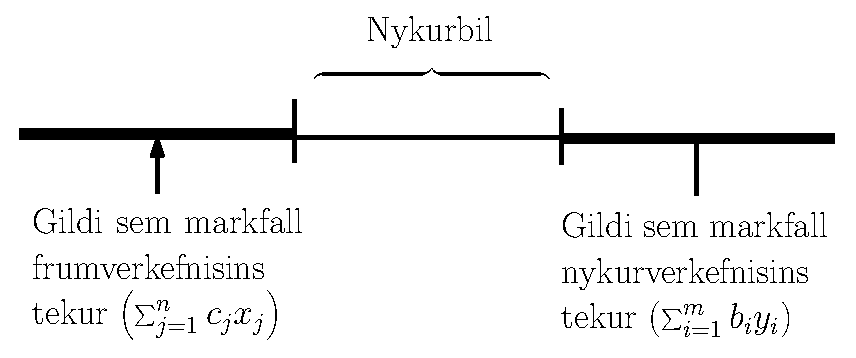
\includegraphics[width=0.6\columnwidth]{figs/nykurbil.eps}
\end{figure}
\begin{setn}[\ath{Sterka nykursetningin} (e. strong duality theorem)] Ef $\vec{x}^*=(x_1^*,...,x_n^*)$ er besta lausn á frumverkefninu. Þá er $\vec{y}^*=(y_1^*,...,y_m^*)$ besta lausn nykurverkefnisins og 
$$\vec{c}^T\vec{x}^*=\vec{b}^T\vec{y}^*$$
 \end{setn}
 Setningin segir að ef til er besta lausn á frumverkefninu þá er ekkert nykurbil. 
Höfum því fjóra möguleika
\begin{enumerate}
 \item Besta lausn til á bæði frum og nykur (ekkert bil)
 \item Frum ótakmarkað, nykur ógjaldgengt (ekkert bil)
 \item Frum ógjaldgengt, nykur ótakmarkað (ekkert bil)
 \item Bæði frum og nykur ógjaldgeng (óendanlegt bil)
\end{enumerate}
\begin{samepage}
\begin{aths}\hspace{.1cm}
 \begin{enumerate}
  \item Efri og neðri mörk á markfalli geta komið að margvíslegum notum, t.d.
 \begin{enumerate}[label=(\roman{*})]
  \item Til að ákvarða hvenær á að stoppa bestunarreiknirit (t.d. innri punkta aðferðir)\\
  $\rightarrow$ stopp þegar $\left|\vec{b}^T\vec{y}-\vec{c}^T\vec{x}\right|\leq \epsilon$, þar sem $\epsilon>0$ er lítil tala.
  \item Takmarka lausnarsvæði í heiltölubestun (sjá kafla \ref{ch:ip}).
 \end{enumerate}
 \item Í endurbættri Simplex-aðferðinni skiptir fjöldi skorða ($m$) meira máli en fjöldi breyta ($n$) fyrir tímann sem útreikningar taka. Þess  vegna getur verið hagkvæmara að leysa nykurverkefnið ef $m\gg n$.
 \end{enumerate}
\end{aths}
\end{samepage}
\begin{samepage}
\begin{daemi}\label{daemi:frum}
Fyrirtækið \emph{Frum} framleiðir tækjabúnað og glingur.
\begin{enumerate}
\item Eitt kíló af tækjabúnaði þarfnast 1 vinnustundar, 1 einingu af timbri, 2 einingar af málmi, og er þá hagnaðurinn 5 evrur.
\item Eitt kíló af glingri  þarfnast 2 vinnustunda, 1 einingu af timbri, 1 einingar af málmi, og hagnaðurinn er þá 4 evrur.
\item Tiltækar vinnustundir eru 120, 70 einingar af timbri og 100 einingar af málmi.
\end{enumerate}
Hversu mikið af tækjabúnaði $x_1$ og glingri $x_2$ á fyrirtækið að framleiða til að hámarka hagnað? 
\end{daemi}
\end{samepage}

\begin{lausn}Línuleg bestunarverkefni fyrir \emph{Frum} er eftirfarandi 
$$ \mbox{Hámarka hagnað:} \quad \max_{x_1,x_2} z = 5 x_1 + 4 x_2  \mbox{ (evrur) }  $$
m.t.t. sk. 
\[ \begin{array}{lrcl}
\mbox{Vinnustundir:} & x_1 + 2 x_2 &\le& 120 \\
\mbox{Timbur:} & x_1 + x_2 &\le &70  \\
\mbox{Málmur:}& 2x_1 + x_2 &\le& 100 \\
& x_1, x_2 &\ge& 0 
\end{array}\]
\end{lausn}

\begin{daemi}\label{daemi:nykur}
Fyrirtækið \emph{Nykur} vill bjóða í hráefnin sem \emph{Frum}
á og er til í að kaupa hvaða magn sem er. Hvaða verð á
\emph{Nykur} að bjóða þannið að \emph{Frum} selji allt hráefnið?

Látum $y_1$, $y_2$, $y_3$ vera verðin fyrir eina
vinnustund, eina einingu af timbri og eina einingu af málmi.
Verðin þurfa að vera nógu há þannig að það borgi sig fyrir
\emph{Frum} að selja frekar en að framleiða tækjabúnað og glingur, þ.e.a.s.
$y_1+y_2+2y_3\ge 5 \mbox{ og } 2y_1+y_2+y_3\ge 4$.

Fyrirtækið \emph{Nykur} vill vitaskuld ekki greiða of mikið,
þannig fáum við nýtt (nykur-)verkefni.
\end{daemi}
\begin{lausn}
$$\textrm{Lágmarka verð:}\quad\min_{y_1,y_2,y_3} w = 120 y_1 + 70 y_2 + 100 y_3  \mbox{ (evrur)}  $$
m.t.t. sk.
\[ \begin{array}{lrclc}
\mbox{Tækjabúnaður:} & y_1 + y_2 + 2y_3 &\ge& 5 & \mbox{ (evrur)}\\
\mbox{Glingur:} & 2y_1 + y_2 + y_3 &\ge& 4 & \mbox{ (evrur)}\\
 & y_1, y_2, y_3 &\ge& 0 
   \end{array}
\]
 \end{lausn}
\begin{samepage}
Skoðum nú sambandið á milli lausna frum- og nykurverkefna.
\begin{lausn}[á dæmum \ref{daemi:frum} og \ref{daemi:nykur}]
Fyrst lítum við á frumverkefnið leyst með Simplex aðferðinni:
{\scriptsize
\[\begin{array}{|c|ccccc|c|}\hline
z & x_1 & x_2 & x_3 & x_4 & x_5 & HH\\ \hline 
     1 & -5 & -4 &  0 &  0 &  0 &  0 \\
     0 &  1 &  2 &  1 &  0 &  0 &  120 \\
     0 &  1 &  1 &  0 &  1 &  0 & 70 \\
     0 &  2 &  1 &  0 &  0 &  1 &  100 \\ \hline 
\multicolumn{7}{l}{>> T=pivot(T,4,2)} \\  \hline 
    1 & 0 &-1.5 & 0 & 0 & 2.5 &  250 \\
    0 & 0 & 1.5 & 1 & 0 &-0.5 &  70 \\
    0 & 0 & 0.5 & 0 & 1 &-0.5 &  20 \\
    0 & 1 & 0.5 & 0 & 0 & 0.5 &  50 \\ \hline 
\multicolumn{7}{l}{>> T=pivot(T,3,3)} \\ \hline 
     1  &   0  &   0  &   0  &   3 &    1 &  310 \\
     0  &   0  &   0  &   1  &  -3 &    1 &   10 \\
     0  &   0  &   1  &   0  &   2 &   -1 &   40 \\
     0  &   1  &   0  &   0  &  -1 &    1 &   30 \\ \hline
  \end{array}\]}
Lesum úr lokatöflunni:
\begin{eqnarray*}
 \vec{x}^* &=&  (30, 40, 10, 0, 0) \\ z^* &=& 310 \\ \vec{y}^* &=& (0, 3, 1)
\end{eqnarray*}
\end{lausn}
\end{samepage}
Leysum nú nykurverkefnið með stóru $M$-aðferðinni í \textsc{matlab}:
\begin{lstlisting}
>> syms M
>> format rational
>> Tdual=[-1 b' zeros(1,n) M M 0; zeros(n,1) A' -eye(n) eye(n) c]
 
Tdual =
 
[ -1, 120, 70, 100,  0,  0, M, M, 0]
[  0,   1,  1,   2, -1,  0, 1, 0, 5]
[  0,   2,  1,   1,  0, -1, 0, 1, 4]
 
>> Tdual = pivot(Tdual,2,7) % Koma grunnbr x6 a eiginlegt form
 
Tdual =
 
[ -1, 120 - M, 70 - M, 100 - 2*M,  M,  0, 0, M, -5*M]
[  0,       1,      1,         2, -1,  0, 1, 0,    5]
[  0,       2,      1,         1,  0, -1, 0, 1,    4]
 
>> Tdual = pivot(Tdual,3,8) % Koma grunnbr x7 a eiginlegt form
 
Tdual =
 
[ -1, 120 - 3*M, 70 - 2*M, 100 - 3*M,  M,  M, 0, 0, -9*M]
[  0,         1,        1,         2, -1,  0, 1, 0,    5]
[  0,         2,        1,         1,  0, -1, 0, 1,    4]
 
>> % Hefjum Simplex-bestun --------------------------------------
>> Tdual = pivot(Tdual,2,4)
 
Tdual =
 
[-1,70-(3*M)/2, 20-M/2, 0, 50-M/2, M, (3*M)/2-50, 0,-(3*M)/2-250]
[ 0,       1/2,    1/2, 1,   -1/2, 0,        1/2, 0,         5/2]
[ 0,       3/2,    1/2, 0,    1/2,-1,       -1/2, 1,         3/2]
 
>> Tdual = pivot(Tdual,3,2)
 
Tdual =
 
[ -1, 0, -10/3, 0, 80/3, 140/3, M - 80/3, M - 140/3, -320]
[  0, 0,   1/3, 1, -2/3,   1/3,      2/3,      -1/3,    2]
[  0, 1,   1/3, 0,  1/3,  -2/3,     -1/3,       2/3,    1]
 
>> Tdual = pivot(Tdual,3,3)
 
Tdual =
 
[ -1, 10, 0, 0, 30, 40, M - 30, M - 40, -310]
[  0, -1, 0, 1, -1,  1,      1,     -1,    1]
[  0,  3, 1, 0,  1, -2,     -1,      2,    3]
 
>> % Bestun lokid; tokum ut gervibreytur
 
Tdual =
 
[ -1, 10, 0, 0, 30, 40, -310]
[  0, -1, 0, 1, -1,  1,    1]
[  0,  3, 1, 0,  1, -2,    3] 
\end{lstlisting}
Lesum úr lokatöflunni:
\begin{eqnarray*}
 \vec{y}^* &=& (0, 3, 1,0,0)\\ z^* &=& 310 \\ \vec{x}^* &=&  (30, 40) 
\end{eqnarray*}

\begin{figure}[t!]
\centering
 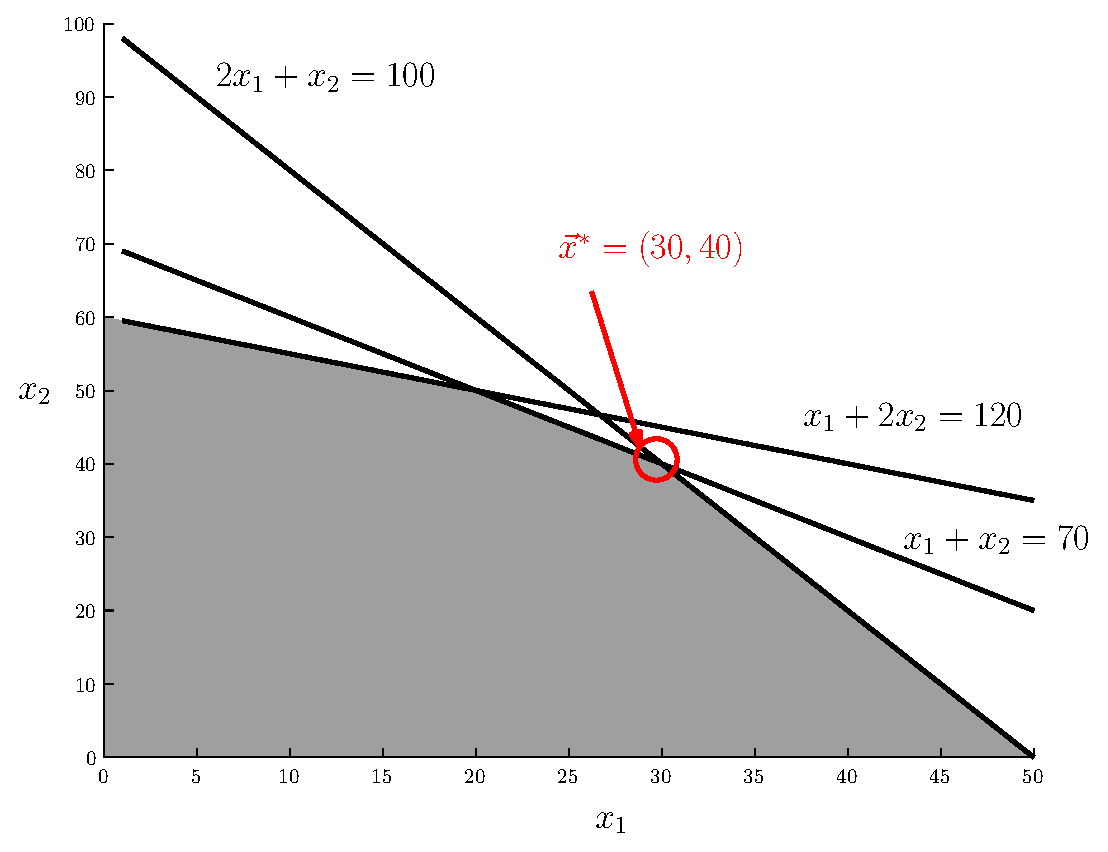
\includegraphics[width=0.85\columnwidth]{figs/wyndor_frumlausn.eps}
 \caption{Myndræn lausn á frumverkefninu \ref{daemi:frum}} 
 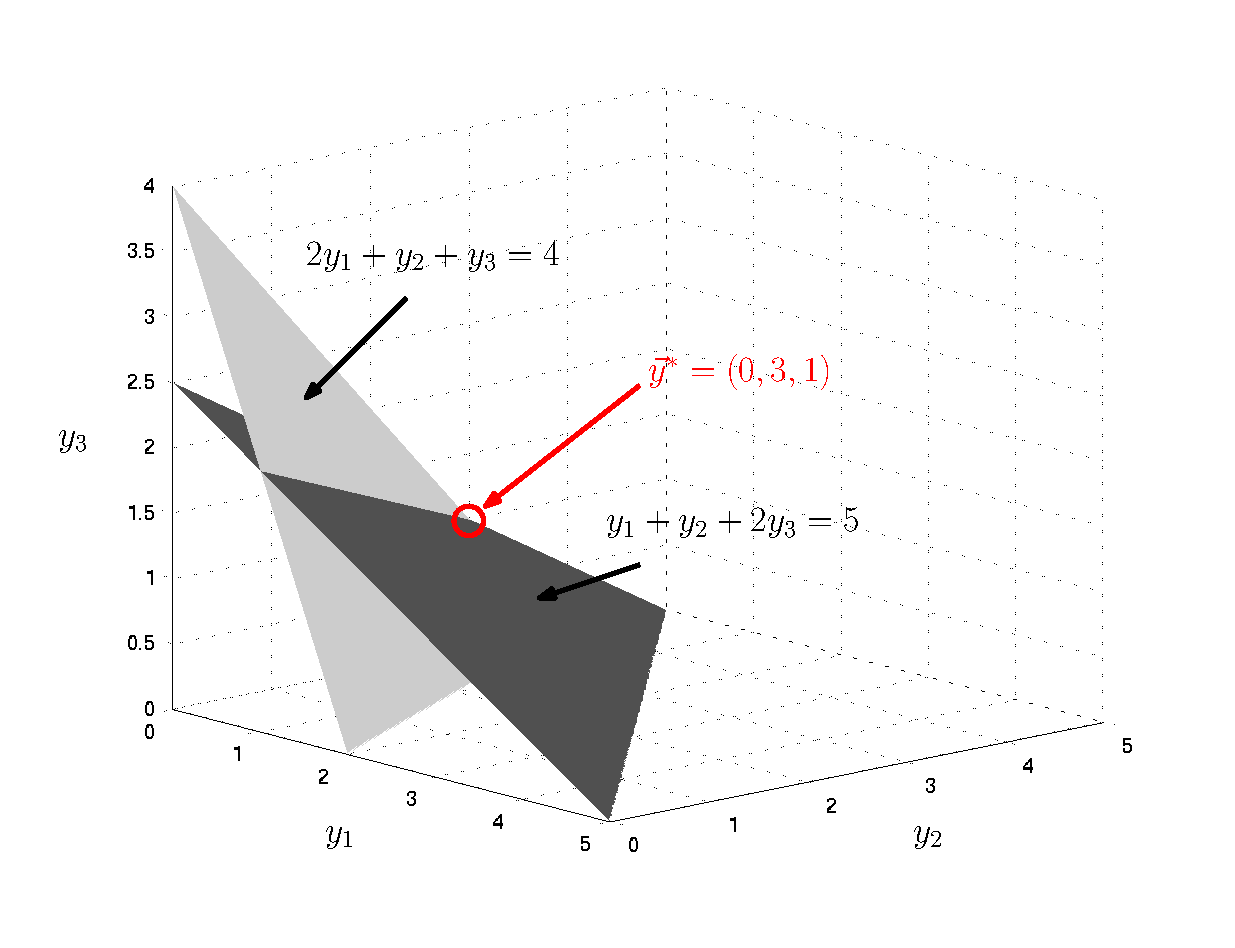
\includegraphics[width=0.85\columnwidth]{figs/wyndor_nykurlausn.eps}
 \caption{Myndræn lausn á nykurverkefninu \ref{daemi:nykur}} 
\end{figure}
%\end{lausn}

\begin{samepage}
\section{Hagfræðileg túlkun nykurverkefna}
Um frumverkefnið gildir
\begin{itemize}
 \item[$x_j$] Magn sem framleitt er af vöru (e. activity) $j$, $j\in\{1,...,n\}$.
 \item[$c_j$] Framlegð af vöru $j$ (á einingu).
 \item[$z$] Heildarhagnaður.
 \item[$b_i$] Magn af hráefni (e. resource) $i$ sem er til ráðstöfunar, $i\in\{1,...,m\}$.
 \item[$a_{ij}$] Magn af hráefni $i$ sem þarf til þess að framleiða eina einingu af vöru $j$.
\end{itemize}
Í sérhverri ítrun er gildi markfallsins
$$w=\sum_{i=1}^m b_iy_i$$
þ.e. framlag $b_i$ eininga af hráefni til markfallsins er $y_ib_i$ og því má túlka $y_i$ sem framlag einnar einingar af hráefni $i$ til markfallsins. Gildin á $y_i$ ($y_i^*$ í bestu lausn) kallast \ath{skuggaverð} (e. shadow price), $y_i^*=\frac{\partial w^*}{\partial b_i}$.

Við framleiðslu á vöru $j$ eru notaðar $a_{ij}$ einingar af hráefni $i$ og $\sum_{i=1}^m a_{ij}y_i$ er því framlag til markfalls af \emph{hráefnisblöndunni} sem þarf til að framleiða eina einingu af vöru $j$. Þessa hráefnisblöndu mætti einnig nota við framleiðslu á öðrum vörum. Það er einungis skynsamlegt ef $\sum_{i=1}^m a_{ij}y_i\geq c_j$ (annars værum við ekki að nota hráefnin á hagkvæmasta máta).
\end{samepage}
\section{Tengsl frum- og nykurverkefna}
%\footnotetext{skoðið líka töflurnar í kafla 6.4 H\&L}
\begin{description}
 \item[\ath{Frumverkefni} $P$] (e. primal):
\begin{eqnarray*}
\max & z = \sum_{j=1}^n c_j x_j & \\
\mbox{sk.} & \sum_{j=1}^n a_{ij}x_j \le b_i, & i \in \mathcal{I}_1\\
 & \sum_{j=1}^n a_{ij}x_j \ge b_i, & i \in \mathcal{I}_2\\
 & \sum_{j=1}^n a_{ij}x_j = b_i, & i \in \mathcal{I}_3 \\
 & x_j \ge 0, & j \in \mathcal{J}_1  \\
 & x_j \le 0, & j \in \mathcal{J}_2  \\
 & x_j \ ^>_<\  0, & j \in \mathcal{J}_3  
\end{eqnarray*}
 \item[\ath{Nykurverkefni} $D$] (e. dual):
\begin{eqnarray*}
\min & w = \sum_{i=1}^m b_i y_i & \\
\mbox{sk.} & \sum_{i=1}^m a_{ij}y_i \ge c_j, & j \in \mathcal{J}_1\\
 & \sum_{i=1}^m a_{ij}y_i \le c_j, & j \in \mathcal{J}_2\\
 & \sum_{i=1}^m a_{ij}y_i = c_j, & j \in \mathcal{J}_3 \\
 & y_i \ge 0, & i\in \mathcal{I}_1  \\
 & y_i \le 0, & i\in \mathcal{I}_2  \\
 & y_i \ ^>_<\  0, & i \in \mathcal{I}_3  
\end{eqnarray*}
\end{description}

\begin{aths}Um gagnvirk verkefni gildir:
\begin{itemize}
\item Til sérhverra skorðu í ($P$) svarar nykurbreyta.
\item Til sérhverra skorðu í ($D$) svarar frumbreyta.
\item Stuðlar markfalls ($P$) eru hægri hlið (HH) í ($D$)
\item Stuðlar markfalls ($D$) eru HH í ($P$)
\item Gagnvirkt (nykur) verkefni gagnvirka verkefnisins er upphaflega (frum) verkefnið, þ.e. nykur af nykur er frum. 

\begin{lausn}
{\scriptsize
\begin{eqnarray*}
\begin{array}{lc} \max & \vec{c}^T\vec{x}\\ \textrm{sk.}&\vec{A}\vec{x}\leq \vec{b} \\ & \vec{x}\geq\vec{0}\end{array}
&\stackrel{\textrm{nykur}}{\rightarrow}&
\begin{array}{lc} \min & \vec{b}^T\vec{y}\\ \textrm{sk.}&\vec{y}^T\vec{A}\geq \vec{c} \\ & \vec{y}\geq\vec{0}\end{array} 
\stackrel{\textrm{staðlað form}}{\rightarrow}
\begin{array}{lc} \max & -\vec{b}^T\vec{y}\\ \textrm{sk.}&-\vec{y}^T\vec{A}\leq -\vec{c} \\ & \vec{y}\geq\vec{0}\end{array} 
\\&\stackrel{\textrm{nykur}}{\rightarrow}&
\begin{array}{lc} \min & -\vec{c}^T\vec{x}\\ \textrm{sk.}&-\vec{A}\vec{x}\geq -\vec{b} \\ & \vec{x}\geq\vec{0}\end{array} 
\stackrel{\textrm{staðlað form}}{\rightarrow}
\begin{array}{lc} \max & \vec{c}^T\vec{x}\\ \textrm{sk.}&\vec{A}\vec{x}\leq \vec{b} \\ & \vec{x}\geq\vec{0}\end{array}  
\end{eqnarray*}}\end{lausn}
Það skiptir því ekki máli hvort verkefnið við köllum frum eða nykur. Venjan er þó að kalla verkefnið sem við setjum (fyrst) fram, frumverkefni. 
\item Stundum er mun ódýrara að leysa gagnvirk (nykur) verkefni en það upphaflega (frum). Það gildir þegar skorður eru mun fleiri en fjöldi breyta, $m \gg n$.
\item $w^* = \vec{y}^*\vec{b}  = \vec{c}^T \vec{x}^* = z^*$ (notum $^*$ til að tákna bestu lausn, sjá líka bls. 201 í H\&L, e. strong duality property).
\item Ef $\vec{x}$ er gjaldgeng lausn í frumverkefninu og $\vec{y}$ er leyfileg lausn í nykur\-verkefninu þá er $\vec{c}^T\vec{x}\le \vec{y}\vec{b}$ (e. weak duality property).
\item Í hverri ítrun simplex aðferðarinnar þá er fundin leyfileg grunnlausn (BFS) $\vec{x}$ og samsvarandi $\vec{y}$ fyrir nykurverkefnið, $\vec{c}\vec{x}=\vec{y}\vec{b}$ (e. complementary solution property). Ef $\vec{x}$ er ekki besta lausn í ($P$) þá er $\vec{y}$ ekki gjaldgeng lausn í ($D$).
\end{itemize}
\end{aths}


Rifjum upp Simplex-töfluna á fylkjaformi (fyrir hvaða ítrun sem er):
\begin{center}
{\renewcommand{\arraystretch}{1.5} \renewcommand{\tabcolsep}{0.2cm}{\footnotesize
\[ \begin{array}{|cc|c|cc|c|}\hline 
  \textrm{Grunnbr.} & \textrm{Jafna} & z & \textrm{Upphafl. br.} & \textrm{Slakabr.} & \textrm{Hægri hlið} \\ \hline\hline
  z & (0) & 1 & \vec{c}_B\vec{B}^{-1}\vec{A}-\vec{c} & \vec{c}_B\vec{B}^{-1} & \vec{c}_B\vec{B}^{-1}\vec{b} \\
\vec{x}_B & (1,\ldots,m) & \vec{0} & \vec{B}^{-1}\vec{A} & \vec{B}^{-1} & \vec{B}^{-1}\vec{b} \\ \hline
 \end{array}\]}}\end{center}
Athugum nánar jöfnu $(0)$. Látum $z=\vec{c}_B^T\vec{B}^{-1}\vec{A}=\vec{y}\vec{A}$, þá er $z_j=\sum_{i=1}^m y_i a_{ij}$ og jafna $(0)$ verður
\[ \begin{array}{cccccc|c}
 x_1 & \cdots & x_n & x_{n+1} & \cdots & x_{n+m} & HH \\
 z_1-c_1 & \cdots & z_n-c_n & y_1 & \cdots & y_m & w=\vec{y}^T\vec{b}    
\end{array}\]
Skorða $j$ í nykurverkefninu er $z_j=\sum_{i=1}^m a_{ij}y_i\geq c_j$ (sbr. $\vec{y}^T\vec{A}\geq\vec{c}$) og því má túlka $z_j-c_j$ sem \ath{umframbreytu} (e. surplus variable) fyrir skorðuna (er 0 þegar skorðan er \emph{bindandi}).

Í frumverkefninu fæst grunnlausn m.þ.a. skeyta slakabreytum við $x$-in. Hliðstætt því fæst grunnlausn í nykurverkefni m.þ.a. skeyta umframbreytum við $y$-in, þ.e. $$ (y_1,...,y_m,z_1-c_1,...,z_n-c_n).$$ Nykurverkefni á viðskeyttu formi hefur $n$ breytur í grunni og $m$ utan grunns.

\begin{samepage}
Eftirfarandi samband gildir milli $P$ og $D$
\begin{center}
 \begin{tabular}{lll}
  Frumbreyta 		&	Tilsvarandi nykurbreyta \\ \hline 
  Ákv.br. $x_j$		&	Slakabr. $z_j-c_j$	& $j\in\{1,...,n\}$ \\
  Slakabr. $x_{n+i}$	&	Ákv.br. $y_i$		& $i\in\{1,...,m\}$
 \end{tabular}
\end{center}
Í sérhverri ítrun finnur Simplex-aðferðin gjaldgenga hornpunktslausn $P$ og einnig svonefnda \ath{fyllingalausn} (e. complementary solution) fyrir $D$ þar sem $\vec{c}^T\vec{x}=\vec{b}^T\vec{y}$ (ef $\vec{x}$ er ekki besta lausnin á $P$ þá er $\vec{y}$ ekki gjaldgeng í $D$).
\end{samepage}

\begin{figure}[t!]
\centering
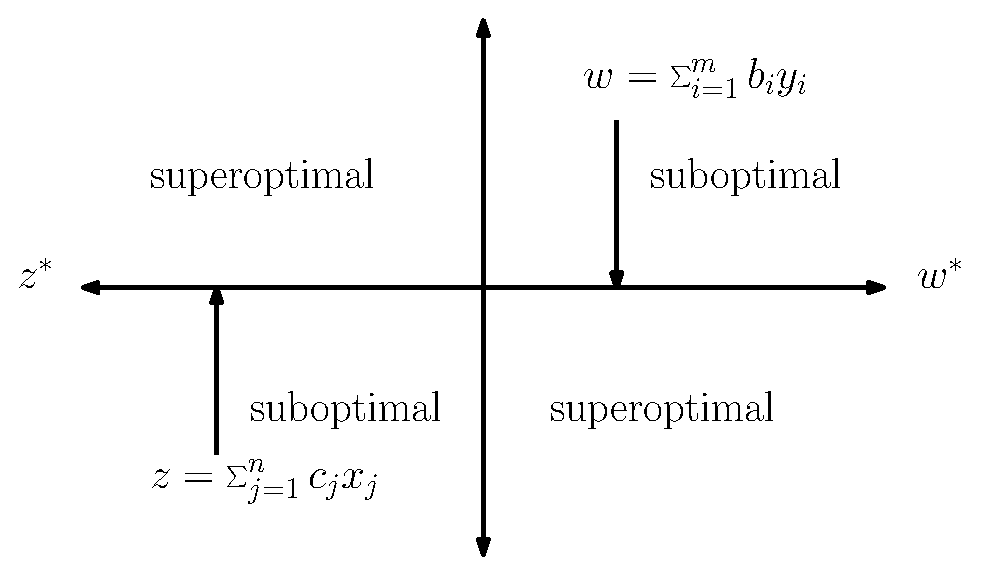
\includegraphics[width=0.7\columnwidth]{figs/complementary.eps}
\end{figure}

Tilsvarandi gildir um grunnlausnir $P$ og $D$. Svarandi til sérhverrar grunn\-lausnar $P$ er \ath{fyllingagrunnlausn} (e. complimentary basic solution) á $D$ og markfallsgildi þeirra ($z$ og $w$) eru þau sömu. Auk þess gildir:
\begin{center}
 \begin{tabular}{ll}
  Frumbreyta 		&	Tilsvarandi nykurbreyta \\ \hline 
  Í grunni $(>0)$	&	Utan grunns $(=0)$	\\
  Utan grunns $(=0)$	&	Í grunni $(>0)$		
 \end{tabular}
\end{center}

Þegar önnur lausnin (frum eða nykur) er þekkt má finna hina með því að leysa jöfnuhneppi.

\begin{setn}[\ath{Complimentary slackness}] Ef $(x_1,...,x_n)$ er besta lausn á $P$ og $(y_1,...,y_m)$ er besta lausn á $D$ þá gildir:
\begin{enumerate}
 \item $x_j(z_j-c_j)=0$ \quad\quad ($z_j-c_j$ er umframbr. í $D$)
 \item $x_{n+1}y_i=0$\quad\quad\quad~~~($x_{n+1}$ er slakabr. í $P$)
\end{enumerate}
fyrir öll $i$ og $j$.
\end{setn}
\begin{proof}Sjáum að strax að 1. og 2. eru tilsvarandi tilvik. 
Höfum að 
\begin{eqnarray*}
\sum_{j=1}^n c_jx_j &\stackrel{(\star)}{\leq}& \sum_{j=1}^n\left(\sum_{i=1}^m a_{ij}y_i\right)x_j
\end{eqnarray*}
því $c_j\leq\sum_{i=1}^m a_{ij}y_i$ (sjá veiku nykursetninguna \ref{setn:veiknykur}).
Jafnaðarmerkið í $(\star)$ gildir annaðhvort þegar
\begin{enumerate}[label=(\roman{*})]
 \item $x_j=0$ fyrir öll $j\in\{1,...,n\}$,
 \item eða $c_j=\sum_{i=1}^m a_{ij}y_i=z_j$ þ.e. $z_j-c_j=0$.
\end{enumerate}
\end{proof}

\section{Frumverkefni sem eru ekki á stöðluðu formi}
Getum alltaf komið línulegu bestunarverkefni yfir á staðlað form 
{\renewcommand{\arraystretch}{1.5} \renewcommand{\tabcolsep}{0.2cm}
\begin{eqnarray*}
 \min z &\rightarrow& \max -z \\
 \vec{a}^T\vec{x}\geq \vec{b} &\rightarrow& -\vec{a}^T\vec{x}\leq-\vec{b} \\
 \vec{a}^T\vec{x}= \vec{b} &\rightarrow& \vec{a}^T\vec{x}\geq \vec{b} \textrm{ og } \vec{a}^T\vec{x}\leq \vec{b} \\
 x_i \textrm{ frjáls } &\rightarrow& x_i=x_i^+-x_i^- \textrm{ með } x_i^+,x_i^-\geq 0.
\end{eqnarray*}}
\begin{aths}
Á bls. 213--215 í H\&L eru nokkur trix sem stytta manni leið við að ákvarða form skorða og breyta í nykurverkefnum. 
\end{aths}
\begin{center}{\renewcommand{\arraystretch}{1.5} \renewcommand{\tabcolsep}{0.2cm}
\begin{tabular}{|ccc|}\hline 
Annað verkefnið && Hitt verkefnið \\ \hline 
$\max z$ (eða $w$) && $\min w$ (eða $z$) \\ \hline
skorða $i$ && breyta $y_i$ (eða $x_i$) \\
$\leq$ &$\longleftrightarrow$& $y_i\geq0$ \\ 
$=$ &$\longleftrightarrow$ & $y_i$ óskorðað \\
$\geq$ &$\longleftrightarrow$& $y_i\leq0$ \\ \hline 
breyta $x_j$ (eða $y_j$) && skorða $j$ \\  
$x_j\geq0$ &$\longleftrightarrow$ & $\geq$ \\ 
$x_j$ óskorðað &$\longleftrightarrow$ & $=$ \\
$x_j\leq0$ &$\longleftrightarrow$& $\leq$ \\ \hline 
\end{tabular}}
\end{center}

\begin{daemi}[Nykurverkefni geisladæmisins \ref{daemi:krabbi}]Höfum frumverkefni:
\begin{center}{\renewcommand{\arraystretch}{1.5} \renewcommand{\tabcolsep}{0.2cm}
\begin{tabular}{|l|rrr|}\hline
Heildarmagn geislunar & \multicolumn{3}{c|}{$\max_{x_1,x_2} -z = -0.4x_1 - 0.5x_2$} \\ \hline
Heilbrigðir vefir & $0.3x_1$ & $+\; 0.1x_2$ & $ \le  2.7 $ \\
Krabbameinssvæði & $ 0.5x_1 $&$ +\; 0.5x_2 $&$=  6.0 $ \\
Miðja æxlis & $0.6x_1$&$ +\; 0.4x_2$& $\ge 6.0$ \\ 
& \multicolumn{3}{c|}{$x_1,x_2 \ge 0$} \\ \hline
\end{tabular}} 
\end{center}
\end{daemi}
\begin{lausn}Þá er nykurverkefnið:
\begin{center}{\renewcommand{\arraystretch}{1.5} \renewcommand{\tabcolsep}{0.2cm}
\begin{tabular}{|l|rrrr|}\hline
&\multicolumn{4}{c|}{$\min_{y_1,y_2,y_3} w = 2.7y_1 + 6y_2+6y_3$} \\ \hline
Geisli 1: & $0.3y_1$ & $+\; 0.5y_2$& $+\; 0.6y_3$ & $ \ge -0.4 $ \\
Geisli 2: & $0.1y_1 $&$ +\; 0.5y_2$& $+\; 0.4y_3$& $ \ge -0.5 $ \\
& \multicolumn{4}{c|}{$y_1 \ge 0$} \\ 
& \multicolumn{4}{c|}{$y_2$ óskorðað}  \\ 
& \multicolumn{4}{c|}{$y_3 \le 0$} \\ \hline
\end{tabular}} 
\end{center} 
\end{lausn}
\section{Strangt fyllingarskilyrði}
Um \ath{ströng fyllingarskilyrði} (e. strict complement\-arity) höfum við: 
\begin{itemize} 
\item Ef strangt fyllingarskilyrði \emph{gildir}, en það segir að allar grunnbreytur séu $\ne 0$ (breytur utan grunns eru jú $0$, en þetta þýðir að engar aðrar breytur séu $0$ \emph{fyrir tilviljun}). Þá gildir: 
  \begin{enumerate}[label=(\roman{*})]
  \item\label{fylli1} $x$ er grunnbreyta þ.þ.a.a. tilsvarandi nykur skorða er virk, þ.e.a.s.
  \begin{eqnarray*}
      x_j\ne 0 & \Longleftrightarrow &\vec{a}_j^T\vec{y} = c_j \\
      x_i^{\mbox{\tiny slaka}} \ne 0 \mbox{  (þ.e. $\vec{a}_i\vec{x}\ne b_i$)} & \Longleftrightarrow & y_i = 0 
   \end{eqnarray*}
   \item\label{fylli2} Ef upphafleg (frum) skorða er virk þ.þ.a.a. tilsvarandi nykur \mbox{breyta} er í grunni, þ.e.a.s. 
  \begin{eqnarray*}
  \vec{a}_i\vec{x} = b_i &\Longleftrightarrow & y_i \ne 0 \\
  x_j = 0  & \Longleftrightarrow & y_j^{\mbox{\tiny slaka}} \ne 0 \mbox{  (þ.e. $\vec{a}_j^T\vec{y}\ne   c_j$)}
  \end{eqnarray*}
  \end{enumerate}
  \begin{aths}Ljóst er að \ref{fylli1} er jafngilt \ref{fylli2}.\end{aths}
  \item Ef strangt fyllingarskilyrði \emph{gildir ekki}, hefur í för með sér að til eru lausnir á frumverkefni og því gagnvirka (nykur):
  \begin{eqnarray*}
  x_j \textrm{ er í grunni } & \Longleftrightarrow & y_j^{\textrm{\textrm{\tiny slaka}}} \textrm{ er utan grunns} \\
  x_i^{\mbox{\tiny slaka}}\textrm{ er í grunni } &\Longleftrightarrow& y_i \textrm{ er utan grunns}  
  \end{eqnarray*}
\begin{aths}Þó skorðan $\vec{a}_j^T\vec{y} = c_j$ sé virk er ekki nauðsynlegt að tilsvarandi slakabreyta sé utan grunns.\end{aths}
\end{itemize}

\section{Næmnigreining og nykurverkefni}\label{sec:naemnigreining}
\ath{Næmnigreining} (e. sensitivity analysis) kannar áhrif breytinga á $c_j, b_i$ og $a_{ij}$ á bestu lausn.
\begin{itemize}
 \item Er lausnin gjaldgeng eftir breytingu?
 \item Er hún enn best?
\end{itemize}
Þessum spurningum (ásamt fleiri) má oft svara með lítilli fyrirhöfn m.þ.a. nýta vensl milli frum- og  nykurverkefna. Sjaldnast þarf að leysa líkanið frá grunni.

\begin{daemi}[Ný vara bætist við hjá Wyndor úr dæmi \ref{wyndor:org}]\label{wyndor:new}
$$\max_{\vec{x}} z= 3x_1+5x_2+4x_{\textrm{ný}} $$
m.t.t. skorðanna
\[\begin{array}{ccccccc}
 x_1 &   &      &+& 2x_{\textrm{ný}} & \leq & 4 \\
     &   & 2x_2 &+& 3x_{\textrm{ný}} & \leq &12 \\
 3x_1& + & 2x_2 &+&  x_{\textrm{ný}} & \leq &18\\
\multicolumn{7}{c}{x_1,x_2,x_{\textrm{ný}}\geq0}
\end{array}\]
Besta lausn sem við fundum fyrir upphaflega verkefnið var \mbox{$x_1=2$},\mbox{$x_2=6$} og því $x_{\textrm{ný}}=0$. Hún er augljóslega gjaldgeng, en er hún enn best?
\end{daemi}
\begin{lausn}Ný breyta í frumverkefni svarar til nýrrar skorðu í nykurverkefni:
\begin{equation}\label{sk:13}
 2y_1+3y_2+y_3\geq4 
\end{equation}
Lesum fyllingalausnina $(\vec{y}^*,\vec{z}^*-\vec{c}^*)=(y_1^*,y_2^*,y_3^*,z_1^*-c_1^*,z_2^*-c_2^*)$ beint út úr loka Simplex-töflunni (sjá lausn á bls. \pageref{wyndor:simplex}):
\begin{center}
{\renewcommand{\arraystretch}{1.5} \renewcommand{\tabcolsep}{0.2cm}
{\scriptsize
$\begin{array}{|c|ccccc|c|} \hline 
\textrm{grunnbr.} &  x_1 &  x_2 &   x_3 &  x_4 &  x_5 &  HH  \\ \hline 
z   &0 & 0 & 0 & \frac{3}{2} & 1 &  36 \\
x_3& 0 & 0 & 1 & \frac{1}{3} & -\frac{1}{3} & 2 \\
x_2& 0 & 1 & 0 & \frac{1}{2} & 0 & 6  \\
x_1& 1 & 0 & 0 &-\frac{1}{3} & \frac{1}{3} & 2  \\ \hline 
\end{array}$
}}\end{center}
þ.e. skorða \eqref{sk:13} fyrir $\vec{y}^*$ verður
$$2\cdot 0+3\cdot \frac{3}{2}+1\cdot1=\frac{11}{2} =5.5\geq 4.$$
Nykurlausnin er gjaldgeng, frumlausnin er gjaldgeng og lausnin er því ennþá best.
\begin{samepage}
\begin{aths}\hspace{.1cm}
  \begin{enumerate}[label=(\roman{*})]
  \item Framlegð $c_{\textrm{ný}}$ er ekki nógu mikil til þess að Wyndor hafi ávinning á því að framleiða þessa nýju vöru.
  \item Önnur leið að sömu niðurstöðu væri að leysa líkanið upp á nýtt.
  \end{enumerate}
\end{aths}\end{samepage}
\end{lausn}

Næmnigreining er mikilvæg í línulegri bestun því gert er ráð fyrri að stikar líkansins ($b_i,c_j,a_{ij}$) eru \emph{þekktir fastar}. Oft eru gildi á stikunum  einhvers konar spá um ástönd sem gilda í framtíðinni (t.d. framlegðartölur) og stikamatið því háð talsverðri óvissu. Í öðrum tilvikum geta gildi á stikunum endurspeglað ákvarðanir sem e.t.v. eru ekki vel ígrundaðar eða væri auðvelt að breyta. Dæmi um slíkt gæti verið tími til umráðana hjá Wyndor.
% Undantekning: Kerfislíffræði
Þess vegna er mikilvægt að kanna hvernig líkanið bregst við breytinum á stikum. Finna þarf hvaða stikar hafa mikil áhrif (e.t.v. þarf að endurmeta einhverja þeirra í framhaldinu). Fyrir þá stika sem hafa tiltölulega lítil áhrif á er gagnlegt að vita á hvaða bili þeir mega liggja án þess að besta lausn breytist að ráði. 

\section{Framgangsmáti næmnigreiningar}
\begin{enumerate}
 \item Uppfæra líkan m.t.t. breytinga á stikum.
 \item Uppfæra loka Simplex-töfluna.
 \item Koma töflunni yfir á eiginlegt form með Gauss-eyðingu.
 \item Er lausnin gjaldgeng? (þ.e. hægri hlið $\geq0$)
\end{enumerate}
\begin{tabular}{llp{10cm}}
\hspace{1cm} & Nei $\rightarrow$ & Besta aftur (laga lokatöflu og nota sem upphafs\-töflu).\\
& Já  $\rightarrow$ & Er lausnin ennþá best? (allir stuðlar í línu $(0)$ eru $\geq 0$)\\
& & Nei $\rightarrow$\quad Ítra með Simplex-aðferðinni.
\end{tabular}

\begin{aths}Ekki er alltaf nauðsynlegt að framkvæma öll þessi skref.\end{aths}

Þessi framgangsmáti miðar við að við viljum framkvæma næmnigreiningu á reikningslega hagkvæman máta, þ.e. ekki leysa líkönin ítrekað frá grunni, fyrir mismunandi gildum á stikunum t.d. $b_1=1,b_1=1.1,b_1=1.2$ o.s.frv.

Við finnum hvernig lokataflan myndi líta út ef við byrjum með nýju gildin $(\overline{\vec{c}},\overline{\vec{b}},\overline{\vec{A}})$ í upphafstöflunni, beitum sömu grunnaðgerðum (Gauss-eyðing) og við gerðum við með upphaflegu gildunum. 
%\begin{aths}Við fengjum líklegast aðra lokatöflu ef við beitum Simplex á $\vec{c},\vec{A}$ og $\vec{b}$.\end{aths}


\begin{table}[h!]
\begin{center}
{\renewcommand{\arraystretch}{1.5} \renewcommand{\tabcolsep}{0.2cm}
\begin{tabular}{|ll|}\hline 
$\overline{\vec{A}}$ & $\vec{A}$ fylki eftir breytingu,\\
$\overline{\vec{b}}$ & hægri hlið eftir breytingu,\\
$\overline{\vec{c}}$ & markfallsstuðlar eftir breytingu,\\
$\vec{y}^*$ & skuggaverð í lokatöflu,\\
$\vec{S}^*$ & stuðlar við slakabreytur í lokatöflu.\\\hline
\end{tabular}}
\caption{Ritháttur}
\end{center}
\end{table}

\begin{samepage}\begin{aths}Algengara er að skoða áhrif þess að breyta einum stika í einu heldur en mörgum í einu.\end{aths}\end{samepage}

\begin{samepage}
Lokatafla eftir breytingar
\begin{center}
{\renewcommand{\arraystretch}{1.5} \renewcommand{\tabcolsep}{0.2cm}
{\footnotesize
\[ \begin{array}{|c|c|cc|c|}\hline 
 \textrm{Jafna} & z & \textrm{Ákv.br.} & \textrm{Slakabr.} & \textrm{Hægri hlið} \\ 
& & x_1,...,x_n & x_{n+1},...,x_{n+m} & \\ \hline
(0) & 1 & \vec{y}^*\overline{\vec{A}}-\overline{\vec{c}} & \vec{y}^* & \vec{y}^*\overline{\vec{b}}=z^* \\
(1,\ldots,m) & \vec{0} & \vec{S}^*\overline{\vec{A}} & \vec{S}^{*} & \vec{S}^{*}\overline{\vec{b}} \\ \hline
 \end{array}\]
}}
\end{center}
\end{samepage}
\subsection{Breytingar á hægri  hlið}
Þegar breytingar eru gerðar á hægri hlið (þ.e. $\vec{b}$) þá er taflan á réttu formi (Gauss-eyðing óþörf), og svo fremi sem hægri hlið er $\geq0$ (gjaldgeng lausn) eftir breytingarnar er lausnin enn best. Hægri hlið verður (eftir breytingu)
 \begin{eqnarray*}
 \textrm{Jafna }(0) \;:& z^*=\vec{y}^*\overline{\vec{b}} \\
 \textrm{Jafna }(1,...,m)\;: & \vec{b}^*=\vec{S}^*\overline{\vec{b}} \\
 \end{eqnarray*}
 \begin{daemi}[Wyndor úr dæmi \ref{wyndor:org}]\label{wyndor:naemni1} Wyndor fer með $b_2$ úr 12 í 24, þ.e. $$\overline{\vec{b}}=\begin{bmatrix}4\\24\\18\end{bmatrix}.$$ Er upphaflega lausnin enn best?
 \end{daemi}
 \begin{lausn}Lokataflan fyrir upphaflega líkanið (sjá lausn á bls. \pageref{wyndor:simplex})
 \begin{center}
{\renewcommand{\arraystretch}{1.5} \renewcommand{\tabcolsep}{0.2cm}
{\scriptsize
$\begin{array}{|c|cc|ccc|c|} \hline 
 Z &  x_1 &  x_2 &   x_3 &  x_4 &  x_5 &  HH   \\ 
\hline\hline 
 1 & 0 & 0 & 0 & \frac{3}{2} & 1 &  36 \\ \hline
 0 & 0 & 0 & 1 & \frac{1}{3} & -\frac{1}{3} & 2 \\
 0 & 0 & 1 & 0 & \frac{1}{2} & 0 & 6  \\
 0 & 1 & 0 & 0 &  -\frac{1}{3} & \frac{1}{3} & 2  \\ \hline 
\end{array}$
}}\end{center} 
Þá verður
\begin{eqnarray*}
 z^*&=&\vec{y}\overline{\vec{b}}=\begin{bmatrix}0 &\frac{3}{2}&1\end{bmatrix}\begin{bmatrix}4\\24\\18\end{bmatrix}=36+18=54\\
 \vec{b}^*&=&\vec{S}^*\overline{\vec{b}}=\begin{bmatrix} 1 & \frac{1}{3} & -\frac{1}{3} \\ 0 & \frac{1}{2} & 0\\ 0 & -\frac{1}{3} & \frac{1}{3}\end{bmatrix}\begin{bmatrix}4\\24\\18\end{bmatrix}=\begin{bmatrix}4+8-6\\12\\-8+6\end{bmatrix}=\begin{bmatrix}6\\12\\-2\end{bmatrix}
\end{eqnarray*}
Lausnin (sem áður var best) er því 
$$ (x_1=-2,x_2=12,x_3=6,x_4=x_5=0)\quad\mbox{með}\quad z=36$$
sem er \emph{ekki gjaldgeng} því $x_1=-2<0$. 

\begin{samepage}
Þurfum því að besta aftur (e. reoptimisation) annaðhvort með
\begin{itemize}
 \item Nykur-Simplex aðferðin (7. kafli), eða 
 \item Frá grunni með $\vec{b}=\begin{bmatrix}4\\24\\18\end{bmatrix}$, 
 \begin{center}
{\renewcommand{\arraystretch}{1.5} \renewcommand{\tabcolsep}{0.2cm}
{\scriptsize
\[\begin{array}{|c|cc|ccc|c|} \hline 
 Z &  x_1 &  x_2 & x_3 & x_4 & x_5 &  HH  \\ \hline\hline 
 1 &  -3 &  -5 &  0 &  0 &  0&  0 \\ 
 0 & 1 &  0 &  1 & 0 & 0 &  4 \\
 0 &  0 &  2 &  0 &   1 &   0 & 24 \\
 0 &  3 &  2 & 0 & 0 & 1 &  18 \\ 
\hline\hline \multicolumn{7}{l}{>> T = pivot(T,4,3)} \\ \hline 
 1 &  \frac{9}{2} & 0 & 0 & 0 & \frac{5}{2}& 45 \\ 
 0 &    1 & 0 & 1 & 0 & 0   & 4 \\ 
 0 &   -3 & 0 & 0 & 1 &-1   & 6 \\ 
 0 &  \frac{3}{2} & 1 & 0 & 0 & \frac{1}{2} & 9 \\ \hline 
\end{array}\]
}}\end{center} \end{itemize}\end{samepage}
Nýja besta lausnin er: $$(x_1=0,x_2=9,x_3=4,x_4=6,x_5=0) \quad\mbox{með}\quad z^*=45.$$ Sjáum að við hættum að framleiða vöru 1.
\end{lausn}
Athugum nú á \emph{hvaða bili} (e. allowable range) $\overline{\vec{b}}$ getur legið þ.a. lausnin verði áfram gjaldgeng
$$\vec{b}^*=\vec{S}^*\overline{\vec{b}}=\vec{S}^*(\vec{b}+\Delta\vec{b})=\vec{S}^*\vec{b}+\vec{S}^*\Delta\vec{b}\geq0$$
\begin{daemi}[Leyfileg breyting á hægri hlið Wyndors]\label{wyndor:naemni2} Sáum í dæmi \ref{wyndor:naemni1} að með $b_2=12\rightarrow24=\overline{b}_2$ varð lausnin óleyfileg. Finnum leyfilega breytingu á $b_2$ þ.a. lausnin verði enn gjaldgeng. 
\end{daemi}
\begin{lausn}Höfum $$\vec{S}^*\Delta\vec{b}=\begin{bmatrix}1 &\frac{1}{3}&-\frac{1}{3}\\0 &\frac{1}{2} & 0\\0&-\frac{1}{3}&\frac{1}{3}\end{bmatrix}\begin{bmatrix}0\\\Delta b_2\\0\end{bmatrix}=\begin{bmatrix}\frac{1}{3}\Delta b_2\\\frac{1}{2}\Delta b_2\\-\frac{1}{3}\Delta b_2\end{bmatrix}$$
Þá þarf að gilda
\[\begin{array}{cccl}
2+\frac{1}{3}\Delta b_2 &\geq 0 & \rightarrow &\Delta b_2\geq-6 \\
6+\frac{1}{2}\Delta b_2 &\geq 0 & \rightarrow &\Delta b_2\geq-12 \\
2-\frac{1}{3}\Delta b_2 &\geq 0 & \rightarrow &\Delta b_2\leq6 
\end{array}\]
Því er $\vec{x}^*$ gjaldgengt ef $-6\leq\Delta b_2\leq 6$, eða $12-6\leq b_2\leq 12+6$, þ.e. $6\leq b_2\leq 18$.
\end{lausn}
\subsection{Breyting á stuðlum ákvarðanabreytu ekki í grunni}\label{breyting:nonbasic}
Breyting á stuðlum við $x_j$, þar sem $x_j$ er ekki í grunni þýðir annaðhvort
$$ a_{ij}\rightarrow \overline{a}_{ij}\quad\mbox{og/eða}\quad c_j\rightarrow\overline{c}_j$$
Lausnin verður áfram gjaldgeng í frumverkefni (því $x_j=0$). Ef hún er líka gjaldgeng í nykurverkefni þá er hún enn best.
\begin{daemi}[Afbrigði af Wyndor]\label{daemi:wyndor:afbrigdi}$$\max_{\vec{x}} z=3x_1+5x_2$$ m.t.t. sk. \[\begin{array}{crl} x_1 & &\leq 4\\&2x_2&\leq24\\3x_1&+2x_2&\leq18\end{array}\]
Besta lausnin var fundin í dæmi \ref{wyndor:naemni2} og var $x_1=0,\;x_2=9$ með $z=45$.
Hvernig breytist lausnin þegar $c_1$ og $a_{i1}$ breytist \emph{samtímis} ef 
$$ c_1=3\rightarrow \overline{c}_1=4\quad\mbox{og}\quad \vec{A}_1=\begin{bmatrix}1\\0\\3\end{bmatrix}\rightarrow\overline{\vec{A}}_1=\begin{bmatrix}1\\0\\2\end{bmatrix}$$
\end{daemi}

\begin{lausn}Lokataflan var fundin hér á undan og var 
  \begin{center}
{\renewcommand{\arraystretch}{1.5} \renewcommand{\tabcolsep}{0.2cm}
{\scriptsize
\[\begin{array}{|c|cc|ccc|c|} \hline 
 Z &  x_1 &  x_2 & x_3 & x_4 & x_5 &  HH  \\ \hline
 1 & \frac{9}{2} & 0 & 0 & 0 & \frac{5}{2}& 45 \\ \hline
 0 &    1 & 0 & 1 & 0 & 0   & 4 \\ 
 0 &   -3 & 0 & 0 & 1 &-1   & 6 \\ 
 0 &  \frac{3}{2} & 1 & 0 & 0 & \frac{1}{2} & 9 \\ \hline 
\end{array}\]
}}\end{center} 
Lesum úr töflunni $y_1^*=0,\;y_2^*=0,\;y_3^*=\frac{5}{2}$ með $z^*=45$.

Ein skorða nykurverkefnisins breytist:
\[\begin{array}{llrcc}
 \mbox{Áður:} & y_1+3y_3 &\geq 3 \\
 \mbox{Eftir:} & y_1+2y_3 &\geq 4  &\stackrel{{\scriptstyle \mbox{set inn } \vec{y}^*}}{\Longrightarrow}& 0+2\frac{5}{2}\geq 4,
\end{array}\]
Lausnin er gjaldgeng í nykurverkefninu, og því enn best.
\end{lausn}

Athugum nú á \emph{hvaða bili} $\overline{\vec{c}}$ getur legið án þess að besta lausn breytist (g.r.f. að $\vec{A}$ breytist ekki). Þá þarf að gilda 
$$z_j^*-c_j\geq0$$ með $z_j^*=\sum_{i=1}^m a_{ij}y_i^*=\vec{y}^*\vec{A}_j$ verður skilyrðið $$c_j\leq \vec{y}^*\vec{A}_j$$
\begin{daemi}[Leyfileg breyting á ekki-grunnbreytu Wyndors]\label{wyndor:naemni3} Á hvaða bili getur $c_1$ legið án þess að besta lausn breytist?  
\end{daemi}
\begin{lausn}
 $$c_i\leq \begin{bmatrix}0&0&\frac{5}{2}\end{bmatrix}\begin{bmatrix}1\\0\\3\end{bmatrix}=1\cdot0+0\cdot0+\frac{5}{2}\cdot3=7.5$$
Leyfilegt bil er því $c_1\leq7.5$.
\end{lausn}
\begin{aths}Stærðin $z_j-c_j$ fyrir breytu $x_j$ sem ekki er í grunni kallast \ath{fallverð} (e. reduced cost). Það segir til um hveru mikill einingakostnaður við vöru $j$ þarf að \emph{lækka} til þess að það borgi sig að framleiða vöruna (þ.e. $x_j$ verði $>0$). 

Ef $c_j$ táknar framlegð/hagnað þá er $z_j-c_j$ hámarks \emph{aukning} á hagnaði þ.a. núverandi grunnlausn sé enn best.
 
\end{aths}

\subsection{Ný breyta innleidd}
Sami framgangsmáti og í \ref{breyting:nonbasic}. Sjá dæmi \ref{wyndor:new}.


\subsection{Breyting á stuðlum ákvarðanabreytu í grunni}
Breyting á stuðlum við $x_j$ þegar $x_j$ er í grunni (í lokatöflu). Eftir að dálkur $j$ hefur verið uppfærður í lokatöflu, þ.e.
\[\begin{array}{lrl}
 \mbox{Stuðullinn við }x_j\mbox{í línu }(0):& z_j^*-\overline{c}_j=&\vec{y}^*\overline{\vec{A}}_j-c_j \\
 \mbox{Stuðlar við }x_j\mbox{í línu }(1,...,m):& \vec{A}_j^*=&\vec{S}^*\overline{\vec{A}}_j
\end{array}\]
þarf yfirleitt að koma töflunni yfir á rétt eiginlegt form með Gauss-eyðingu.
\begin{daemi}[Afbrigði af Wyndor]$$\max_{\vec{x}} z=3x_1+5x_2$$ m.t.t. sk. \[\begin{array}{crl} x_1 & &\leq 4\\&2x_2&\leq24\\3x_1&+2x_2&\leq18\end{array}\]
Besta lausnin var fundin í dæmi \ref{wyndor:naemni2}, og var $(x_1,x_2)=(0,9)$ með $z=45$. Sá möguleiki er fyrir hendi að framlegð vöru 2 hafi verið ofmetin, ásamt því að hráefninotkun hafi verið vanmetin. Könnum áhrif þess að breyta: 
$$ c_2=5\rightarrow \overline{c}_2=3\quad\mbox{og}\quad \vec{A}_2=\begin{bmatrix}0\\2\\2\end{bmatrix}\rightarrow\overline{\vec{A}}_2=\begin{bmatrix}0\\3\\4\end{bmatrix}$$
\end{daemi}
\begin{lausn}Þá er 
\begin{eqnarray*}
 z_2^*-\overline{c}_2 &=& \vec{y}^*\overline{\vec{A}}_2-\overline{c}_2=\begin{bmatrix}0&0&\frac{5}{2}\end{bmatrix}\begin{bmatrix}0\\3\\4\end{bmatrix}-3=10-3=7\\
\vec{A}_2^*&=&\vec{S}^*\overline{\vec{A}}_2=\begin{bmatrix}1 & 0 & 0\\0&0&\frac{1}{2}\\0&1&-1\end{bmatrix}\begin{bmatrix}0\\3\\4\end{bmatrix}=\begin{bmatrix}0\\2\\-1\end{bmatrix}
\end{eqnarray*}
\begin{samepage}
Lokataflan verður þá
\begin{center}
{\renewcommand{\arraystretch}{1.5} \renewcommand{\tabcolsep}{0.2cm}
{\scriptsize
$\begin{array}{|c|ccccc|c|l|} \hline 
 \mbox{grunnbr.} &  x_1 &  x_2 &   x_3 &  x_4 &  x_5 &  HH   & \textrm{minratio-test}\\ 
\hline\hline \multicolumn{7}{l}{>> T } \\ \hline 
 1 & \frac{9}{2} & \bf{7} &  0 &  0 &  \frac{5}{2} &  45 & \mbox{koma á eiginlegt form}\\ 
 x_3 &  1 & 0 &  1 &  0 &  0 &  4 &  \\ 
 x_2 & \frac{3}{2} & \fbox{\bf{2}} &  0 &  0 & \frac{1}{2} & 9 & \\
 x_4 &  -3 & -1 &  0 &  1 &  -1 & 6 & \\ 
\hline\hline \multicolumn{7}{l}{>> T = pivot(T,3,2)} \\ \hline 
 1 & \bf{-\frac{3}{2}} & 0 & 0 &0 & \frac{3}{4} &  \frac{27}{2} & \\
 x_3 & \fbox{1} & 0 & 1 &   0 & 0 & 4 & 4/1=4\leftarrow \min\\
 x_2 & \frac{3}{4} & 1 & 0 & 0 & \frac{1}{4}  & \frac{9}{2} & \frac{9}{2}/\frac{3}{4}=6\\
 x_4 & -\frac{9}{4} & 0 & 0 & 1 & -\frac{3}{4} & 21 & - \\
\hline\hline \multicolumn{7}{l}{>> T = pivot(T,2,1)} \\ \hline 
   1 & 0 & 0 & \frac{3}{4} & 0 & \frac{3}{4} &  \frac{33}{2} &\\
 x_1 & 1 & 0 & 1 & 0 & 0 & 4 &\\
 x_2 & 0 & 1 & -\frac{3}{4} & 0 & \frac{1}{4} & \frac{3}{2} & \\
 x_4 & 0 & 0 & \frac{9}{4} &  1 & -\frac{3}{4} & \frac{39}{2}  & \\ \hline 
\end{array}$
}}\end{center}\end{samepage}
Besta lausn er $x_1^*=\frac{3}{2},\;x_2^*=\frac{3}{2}$ með $z^*=\frac{33}{2}$.
\begin{aths}Besta lausn er \emph{ekki} heiltölulausn!
\end{aths}
\end{lausn}
Það er aðeins meira mál en áður að finna á hvaða bili $c_j$ getur legið þ.a. lausnin sé áfram best. Ástæðan er sú að beita þarf Gauss-eyðingu á lokatöfluna. Sjá bls. 238--239.

\subsection{Ný skorða bætist við}
\begin{itemize}
 \item Ef besta lausn uppfyllir skorðuna, þá er lausnin enn best.
 \item Annars þarf að bæta skorðuna við í lokatöfluna. Koma töfluna yfir á rétt form með Gauss-eyðingu og halda áfram með Simplex.
\end{itemize}
Dæmi um hagnýtingu (kerfislíffræði): Leit að smæsta mengi sem lífverur þurfa að hafa til að geta vaxið og dafnað. Sjá einnig dæmi á bls. 240 í H\&L. 


\subsection{Kerfisbundin næmnigreining}
\ath{Kerfisbundin næmnigreining} (e. parametric programming) skoðar áhrif þess þegar einum eða fleiri stikum er breytt samfellt á einhverju bili.
%\begin{daemi}[Framleiðsla flutt hjá Wyndor] Afköst í verksmiðju 2 er aukin á kostnað verksmiðju 3, þ.a. hún lækkar tvöfalt hraðar en afköstin aukast hjá verksmiðju 2, þ.e.
$$ \max_{\vec{x}} z=3x_1+5x_2$$
m.t.t. sk.
\[\begin{array}{lrrcl}
\mbox{Verksmiðja 1:} & x_1 & &\leq& 4\\
\mbox{Verksmiðja 2:} & & x_2 &\leq& 12+\theta \\
\mbox{Verksmiðja 3:} & 3x_1& +2x_2&\leq& 18-2\theta
\end{array}\]
Könnum áhrif $\theta$ á bestu lausn.
\end{daemi}
\begin{lausn}Breytingar á lokatöflu
\begin{eqnarray*}
 z^*&=&\vec{y}^*\overline{\vec{b}}=\begin{bmatrix}0&\frac{3}{2}&1\end{bmatrix}\begin{bmatrix}4\\12+\theta\\18-2\theta\end{bmatrix}=36-\frac{1}{2}\theta\\
\vec{b}^*&=&\vec{S}^*\overline{\vec{b}}=\begin{bmatrix}1&\frac{1}{3}&-\frac{1}{3}\\0&\frac{1}{2}&0\\0&-\frac{1}{3}&\frac{1}{3}\end{bmatrix}\begin{bmatrix}4\\12+\theta\\18-2\theta\end{bmatrix}=\begin{bmatrix}2+\theta\\6+\frac{1}{2}\theta\\2-\theta\end{bmatrix}
\end{eqnarray*}
Sjáum að öll $\theta\geq0$ minnka hagnað, og lausnin er gjaldgeng þegar $2-\theta\geq0$, þ.e. $\theta \leq 2$.
\end{lausn}
Á hliðstæðan hátt má kanna áhrif þess að breyta markfallsstuðlum samfellt. Í raun er þessi tegund næmnigreiningar áhugaverð þegar
\begin{itemize}
 \item vörur eru í samkeppni innbyrðis,
 \item ytri þættir, t.d. auglýsingar keppinauta, hafa áhrif á framlegðina.
\end{itemize}
\begin{daemi}[Afbrigði af Wyndor]
$$ \max_{\vec{x}} z(\theta)=(3-\theta)x_1+(5-2\theta)x_2$$
m.t.t. sk.
\begin{eqnarray*}
 x_1 &\leq& 4\\
x_2 &\leq& 24\\
3x_1+2x_2&\leq&18\\
x_1,x_2 &\geq&0
\end{eqnarray*}
\end{daemi}
\begin{lausn}Lokatöflu fyrir þetta Wyndor dæmi (áður en $\theta$ var innleitt) sáum við í dæmi \ref{wyndor:naemni1}
 \begin{center}
{\renewcommand{\arraystretch}{1.5} \renewcommand{\tabcolsep}{0.2cm}
{\scriptsize
\[\begin{array}{|c|cc|ccc|c|l|} \hline
  &  x_1 &  x_2 & x_3 & x_4 & x_5 &  HH  &\\ \hline
 z &  \frac{9}{2} & 0 & 0 & 0 & \frac{5}{2}& 45 &\\
 x_3 &    1 & 0 & 1 & 0 & 0   & 4 &\\
 x_4 &   -3 & 0 & 0 & 1 &-1   & 6 &\\
 x_2 &  \frac{3}{2} & 1 & 0 & 0 & \frac{1}{2} & 9 &\\ \hline
\multicolumn{7}{l}{\mbox{Eftir að }\theta\mbox{ hefur verið bætt við}} \\ \hline
 z &  \frac{9}{2}-\theta & \theta & 0 & 0 & \frac{5}{2}& 45 & \mbox{koma á eiginlegt form}\\
 x_3 &    - & - &- & - & -   & - & \mbox{}\\
 x_4 &   - & - & -  & - & -   & - & x_3,x_4\mbox{ skipta ekki máli}\\
 x_2 &  \frac{3}{2} & 1 & 0 & 0 & \frac{1}{2} & 9 &\\ \hline
 z &  \frac{9}{2}-4\theta & 0 & 0 & 0 & \frac{5}{2}-\theta& 45-18\theta & \\
 x_2 &  \frac{3}{2} & 1 & 0 & 0 & \frac{1}{2} & 9 &\\ \hline
\end{array}\]
}}\end{center}
Besta lausn ef
\begin{eqnarray*}
\frac{9}{2}-4\theta\geq0&\Rightarrow &\theta\leq \frac{9}{8}\\
\frac{5}{2}-\theta\geq0&\Rightarrow &\theta\leq \frac{5}{2}\\
\end{eqnarray*}
Svo $\theta\leq \frac{9}{8}$, þ.e. líkanið er ekki sérlega næmt fyrir gildum á $c_1$ og $c_2$.
\begin{aths}Ítarlegri umfjöllun í grein 7.3 í H\&L.\end{aths}

\end{lausn}


\section{Næmnigreining í \textsc{glpk}}

\begin{daemi} Næmnigreining á Wyndor með \athsup{\textsc{glpk}}{Næmnigreining}: Hér ætlum við að taka fyrir gluggabreytuna $x_1$ sér.

\begin{samepage}\lstinputlisting{../glpk/wyndor.mod}\lstinputlisting{../glpk/wyndor.dat}\end{samepage}
\end{daemi}
\newpage
\begin{lausnSYND}
Möguleikinn \texttt{--wcpxlp} býr til skránna \texttt{cplex.txt} sem sýnir hvernig \textsc{glpk} túlkar \textsc{MathProg}. Gott er að skoða þessa skrá til að debögga mögulegar villur -- líka til að athuga hvort líkanið sé ekki örugglega kórrétt:
\lstset{basicstyle=\tiny}
\lstinputlisting{../glpk/wyndor_cplex.txt} 

Keyrum úr skelinni eftirfarandi skipun.
\begin{lstlisting}
glpsol --wcpxlp wyndor_cplex.txt -m wyndor.mod --data wyndor.dat -o wyndor_lausn.txt 
\end{lstlisting}

Næmnigreiningin er síðan í úttaksskránni \texttt{wyndor\_lausn.txt}:
\lstinputlisting{../glpk/wyndor_lausn.txt}

\newpage
Gerum eins fyrir afbrigðið á Wyndor úr dæmi \ref{daemi:wyndor:afbrigdi}
\begin{lstlisting}
hei2@Helga:~/Work/IDN401G/glpk$ glpsol --wcpxlp wyndor_afbrigdi_cplex.txt -m wyndor.mod --data wyndor_afbrigdi.dat -o wyndor_afbrigdi_lausn.txt 
\end{lstlisting}

Næmnigreiningin er síðan í úttaksskránni \texttt{wyndor\_afbrigdi\_lausn.txt}:
\lstinputlisting{../glpk/wyndor_afbrigdi_cplex.txt}
\lstinputlisting{../glpk/wyndor_afbrigdi_lausn.txt}
\lstset{basicstyle=\footnotesize}


\end{lausnSYND}
\section{Samantekt}
Hvernig er lausn verkefnis háð litlum breytingum í
stikum þess $\vec{c}, \mat{A}, \vec{b}$?

\begin{itemize}
\item Hvað er $\frac{\partial z}{\partial c_j}$, $\frac{\partial
    z}{\partial b_i}$, $\frac{\partial z}{\partial a_{ij}}$, ef
  grunnur helst óbreyttur?\\
  
  \underline{Svar}: $\frac{\partial z}{\partial c_j}=x_j$,
  $\frac{\partial z}{\partial b_i}= y_i$, $\frac{\partial
    z}{\partial a_{ij}}=-y_ix_j$ (ekki sannað hérna)\\

\item Hve mikið má breyta $c_j$, $a_{ij}$ og $b_i$ án þess að grunnur breytist?
\end{itemize}

